\paragraph{Overview.}
Blockchains are monolithic solutions for ordering, execution and finality.
We decouple the functionalities, rebranding blockchains as finality-dedicated solutions.
We provide a universal solution for ordering.
We selectively provide case by case optimized solutions for execution.
And we package the whole things back.

Users experience a system that come with order, execution and finality, but without global shared states.
\sys is the platform of applications fulfilling demands involving intersubjectivity, which are inefficient or impossible to be deployed on blockchains.
While supporting different things, \sys has familiar (good) properties to blockchains, both matching users' mind model and enabling easier integrations to present blockchain systems.

\paragraph{Unshared states.}

\begin{figure}[H]
    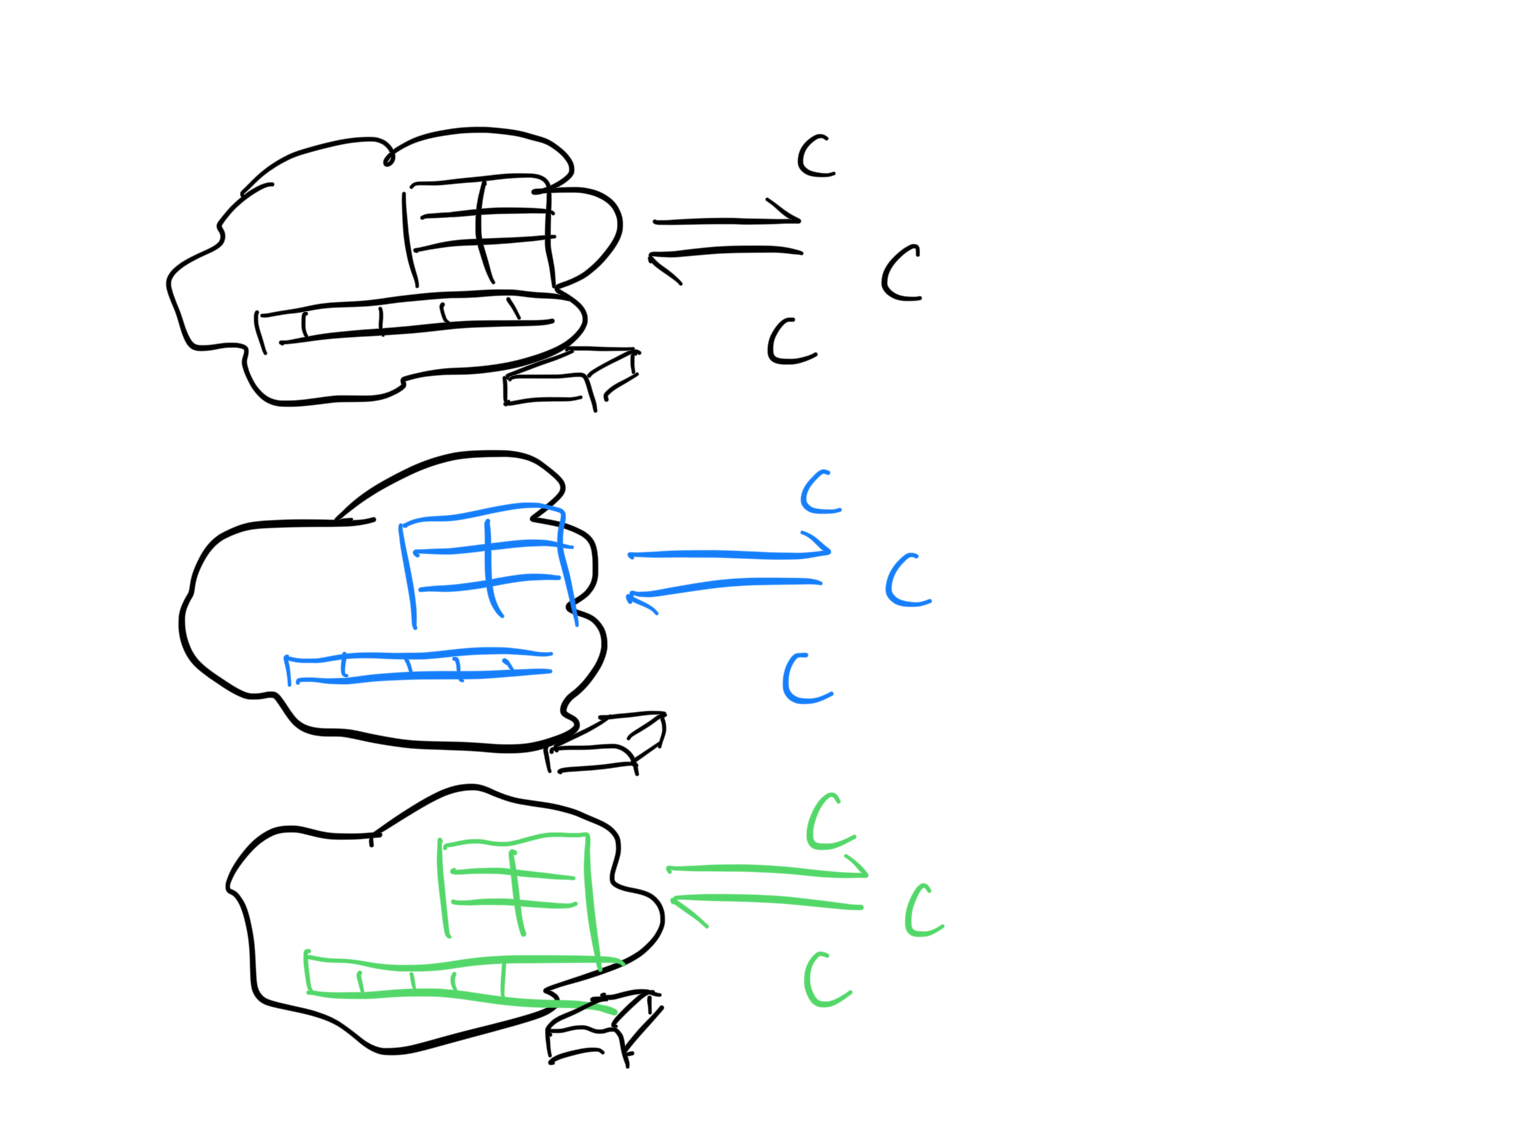
\includegraphics[width=200pt]{graphs/IMG_0060}
    \Description{}
\end{figure}

Making the states unshared essentially brings us back to the centralized solutions, with multiple instances.
The old upsides and downsides are also back.
Let's say we solve the \emph{absolutely faulty} issues with prior solutions.
And the answer to the subjectivities of individual nodes is intersubjectivity.

\begin{figure}[H]
    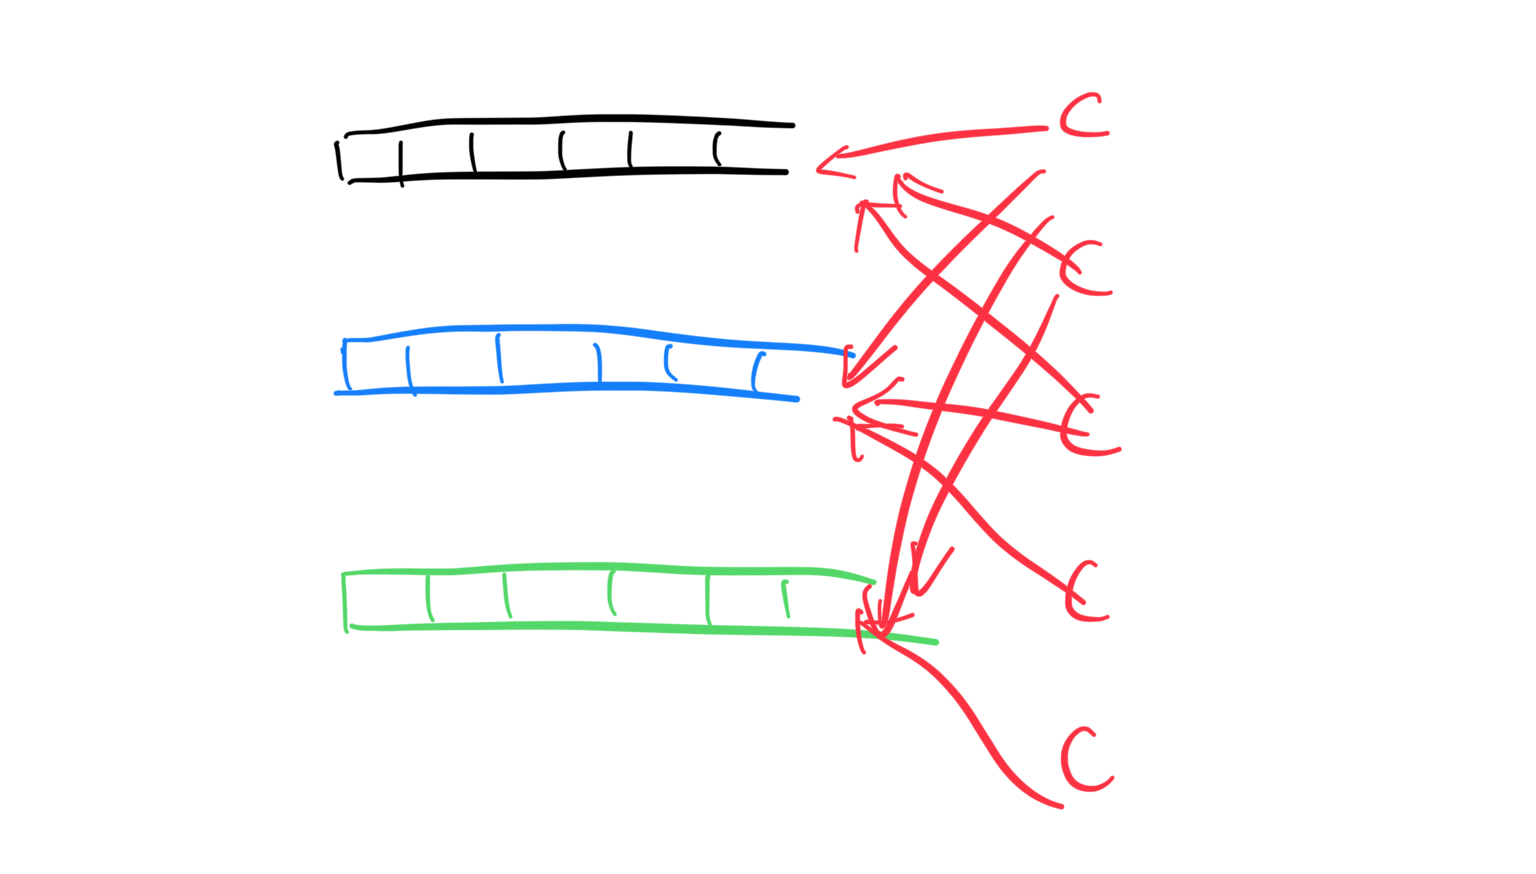
\includegraphics[width=200pt]{graphs/IMG_0059}
    \Description{}
\end{figure}

This approach is aligned with classical financial world, where intersubjectivity is somewhat referred as arbitrage opportunities.

\sgd{In the discussion a broker-centric mechanism is assumed, but here the analogized arbitrage is kind of consumer centric.
Is the possibilities of the system extended by our ``everyone can be the broker'' design?}

But unlike the classical world, where each exchange has external \emph{trust} provided to it that is acknowledged by the other exchanges (which sometimes may not be the case as well), in our setup there's no external source of trust.
There's \emph{no} trust.
By default, nodes will not accept the tokens produced by remote transactions.

As the result, unlike classical exchanges which are the monolithic solutions, the nodes in \sys cannot produce \emph{transactions} in the classical sense.
Transactions are divided into two explicit phases: intention phase and settlement phase.
The intention phase is supported by \sys nodes which are capable for ordering, and the settlement phase is supported by consensus infrastructure \eg blockchains that are capable for providing finality guarantees.
For this reason the nodes of \sys are called \emph{brokers}.

\sgd{We should encourage brokers to colocate consensus nodes with them, to enable a more self-contained system.}

\paragraph{Universal ordering for shared reasoning.}
The explicit intention phase brings unique challenge to \sys compared to the classical financial systems.
In the classical systems, \emph{causality} is the internal detail of the participants: clients judges exchanges locally, and exchanges judges transactions \ie clients locally, the interfaces between clients and exchanges are only transactions and prices.
In \sys however, the transactions are the interfaces between clients and consensus infrastructure, and the \emph{intents}, \ie the \emph{evidences} of why a transaction is later submitted to reach consensus, now become the explicit interfaces between clients and brokers.

In one word, if the communication cannot include transactions directly, it should include the rationales behind the transactions.

\begin{figure}[H]
    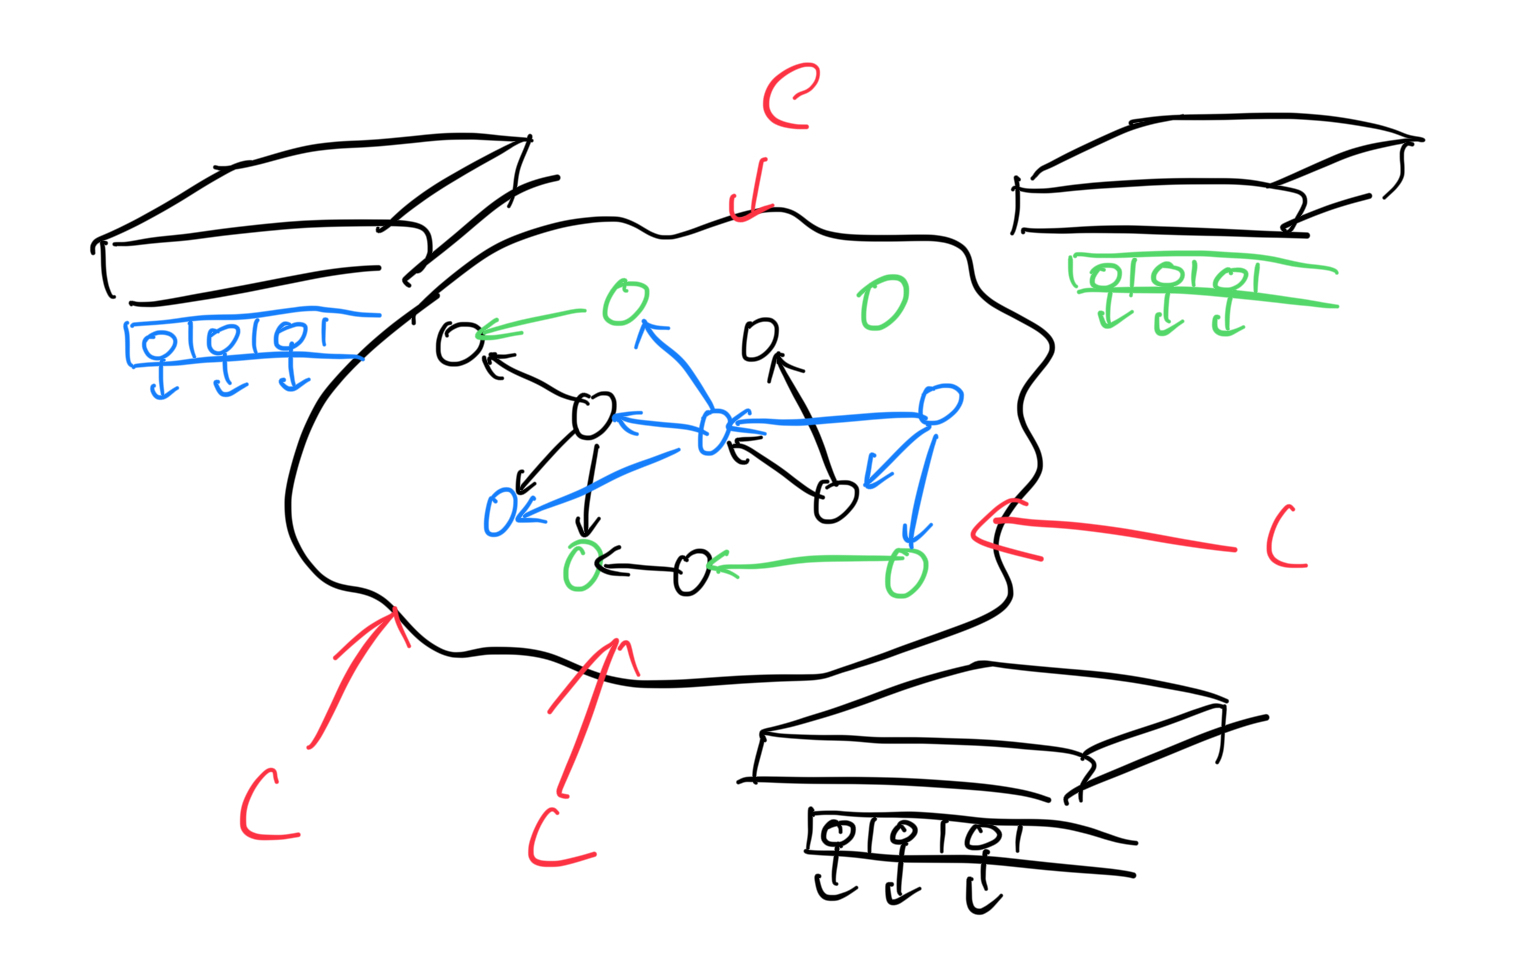
\includegraphics[width=300pt]{graphs/IMG_0058}
    \Description{}
\end{figure}

The intentions are inherently nonlocal.
The most straightforward example is index, where the index price must be tracking (or \emph{happen after}, in causality term) the price of an expected set of things, and the indexers must be able to prove that they do the tracking correctly to convince buyers.
\sgd{Is that ``indexer'' a correct way to say?}
On the other hand, when a transaction involving an index is finalized, each of the indexed thing must be able to prove that it \emph{caused} the index in order to share the profit.
The brokers do not share states, but they must share the relation of their reasoning.

\sys proposes an ordering service to universally connect the reasoning of participants globally, which is
\begin{itemize}
    \item Distributed. 
    \item Independently verifiable.
    \item Append only.
    Upon ordering, everything that the ordered thing is based on must be specified.
    \sgd{Maybe a better representation then talking about causality directly.} 
\end{itemize}

The append-only property enables the ordered intents to be capable to \emph{certify} the reasoning.
In another word, the ordered intents are suitable to be submitted to consensus.

\begin{figure}[H]
    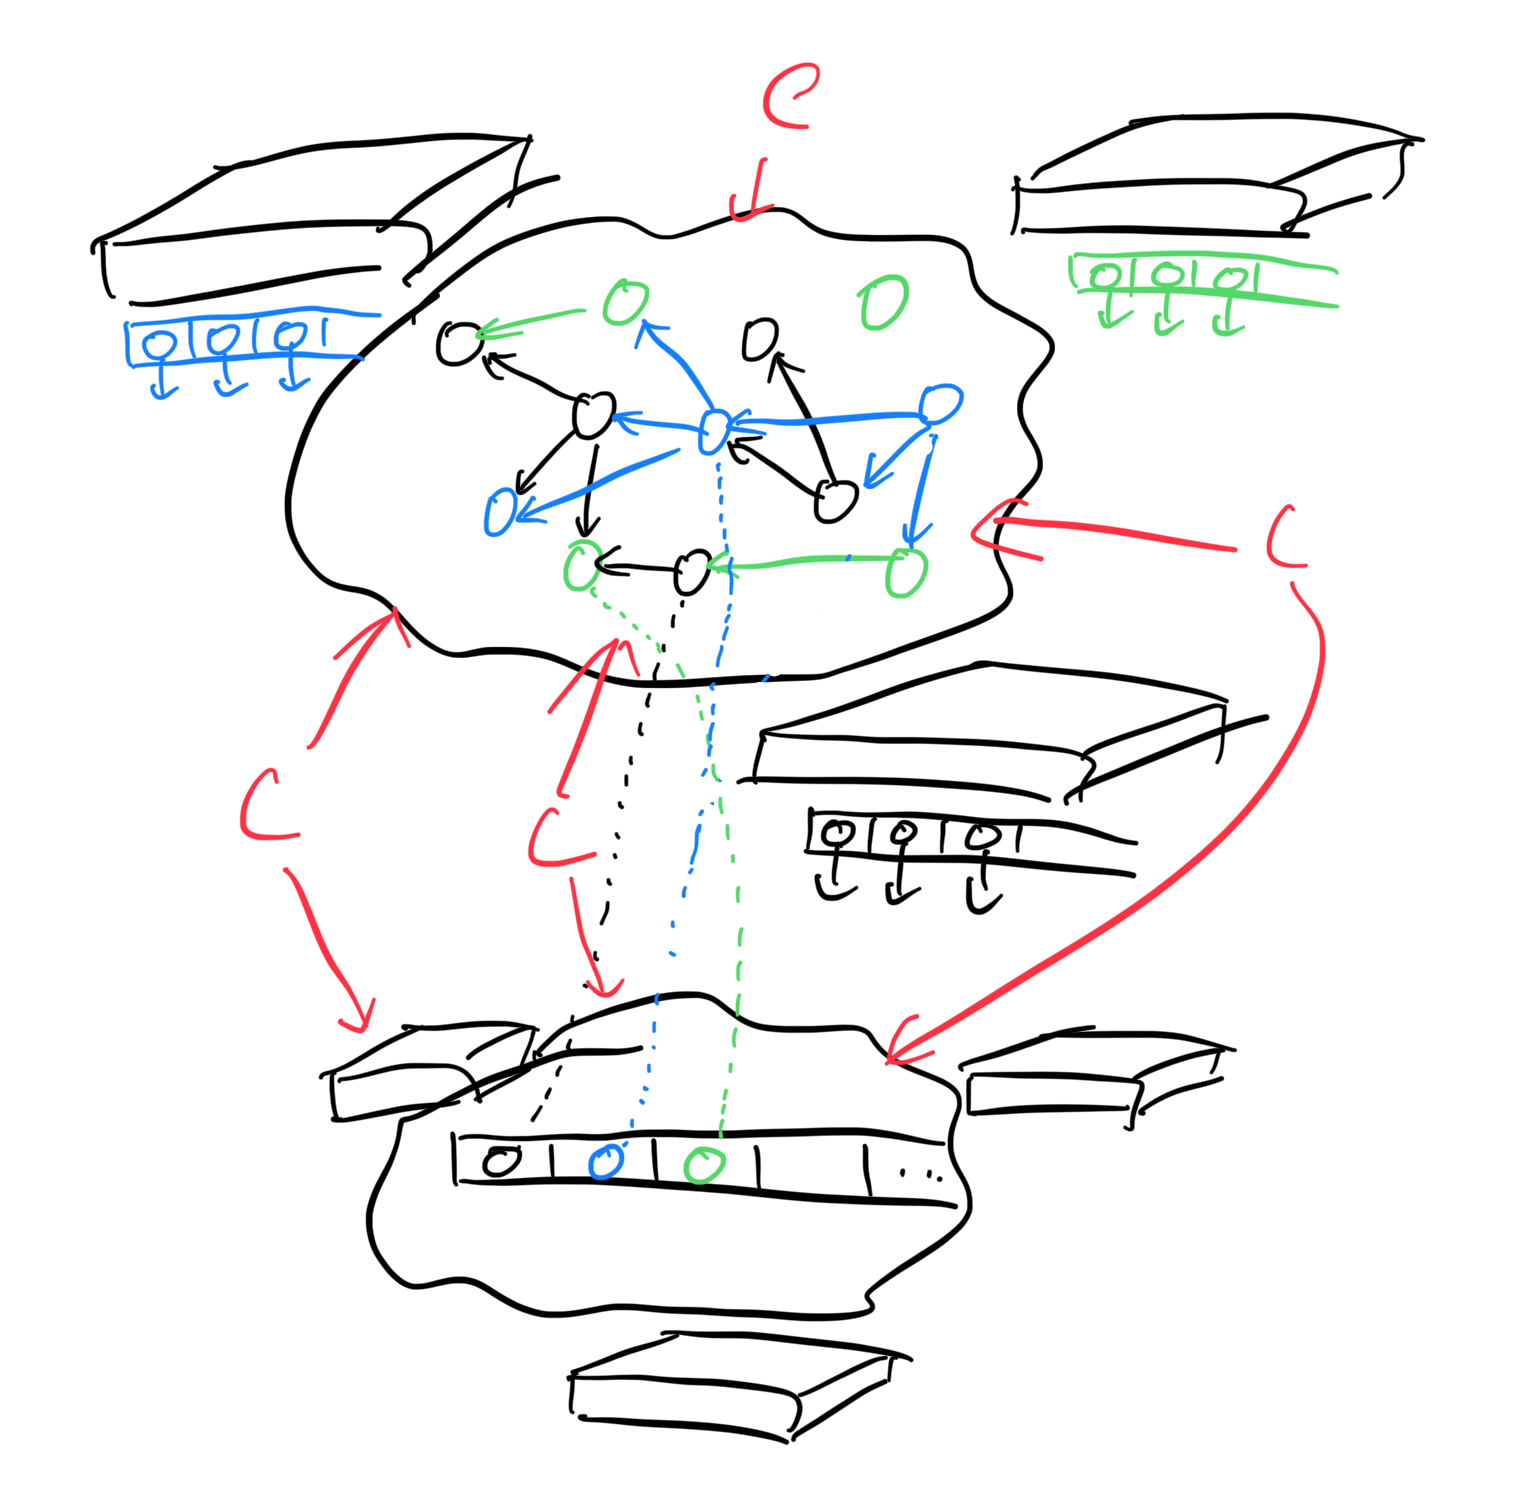
\includegraphics[width=300pt]{graphs/IMG_0056}
    \Description{}
\end{figure}

The finality on the ordered intents is effectively the finality on a \emph{fixed} subset of the based intents - the append-only property prohibits extending the subset retrospectively.

\begin{figure}[H]
    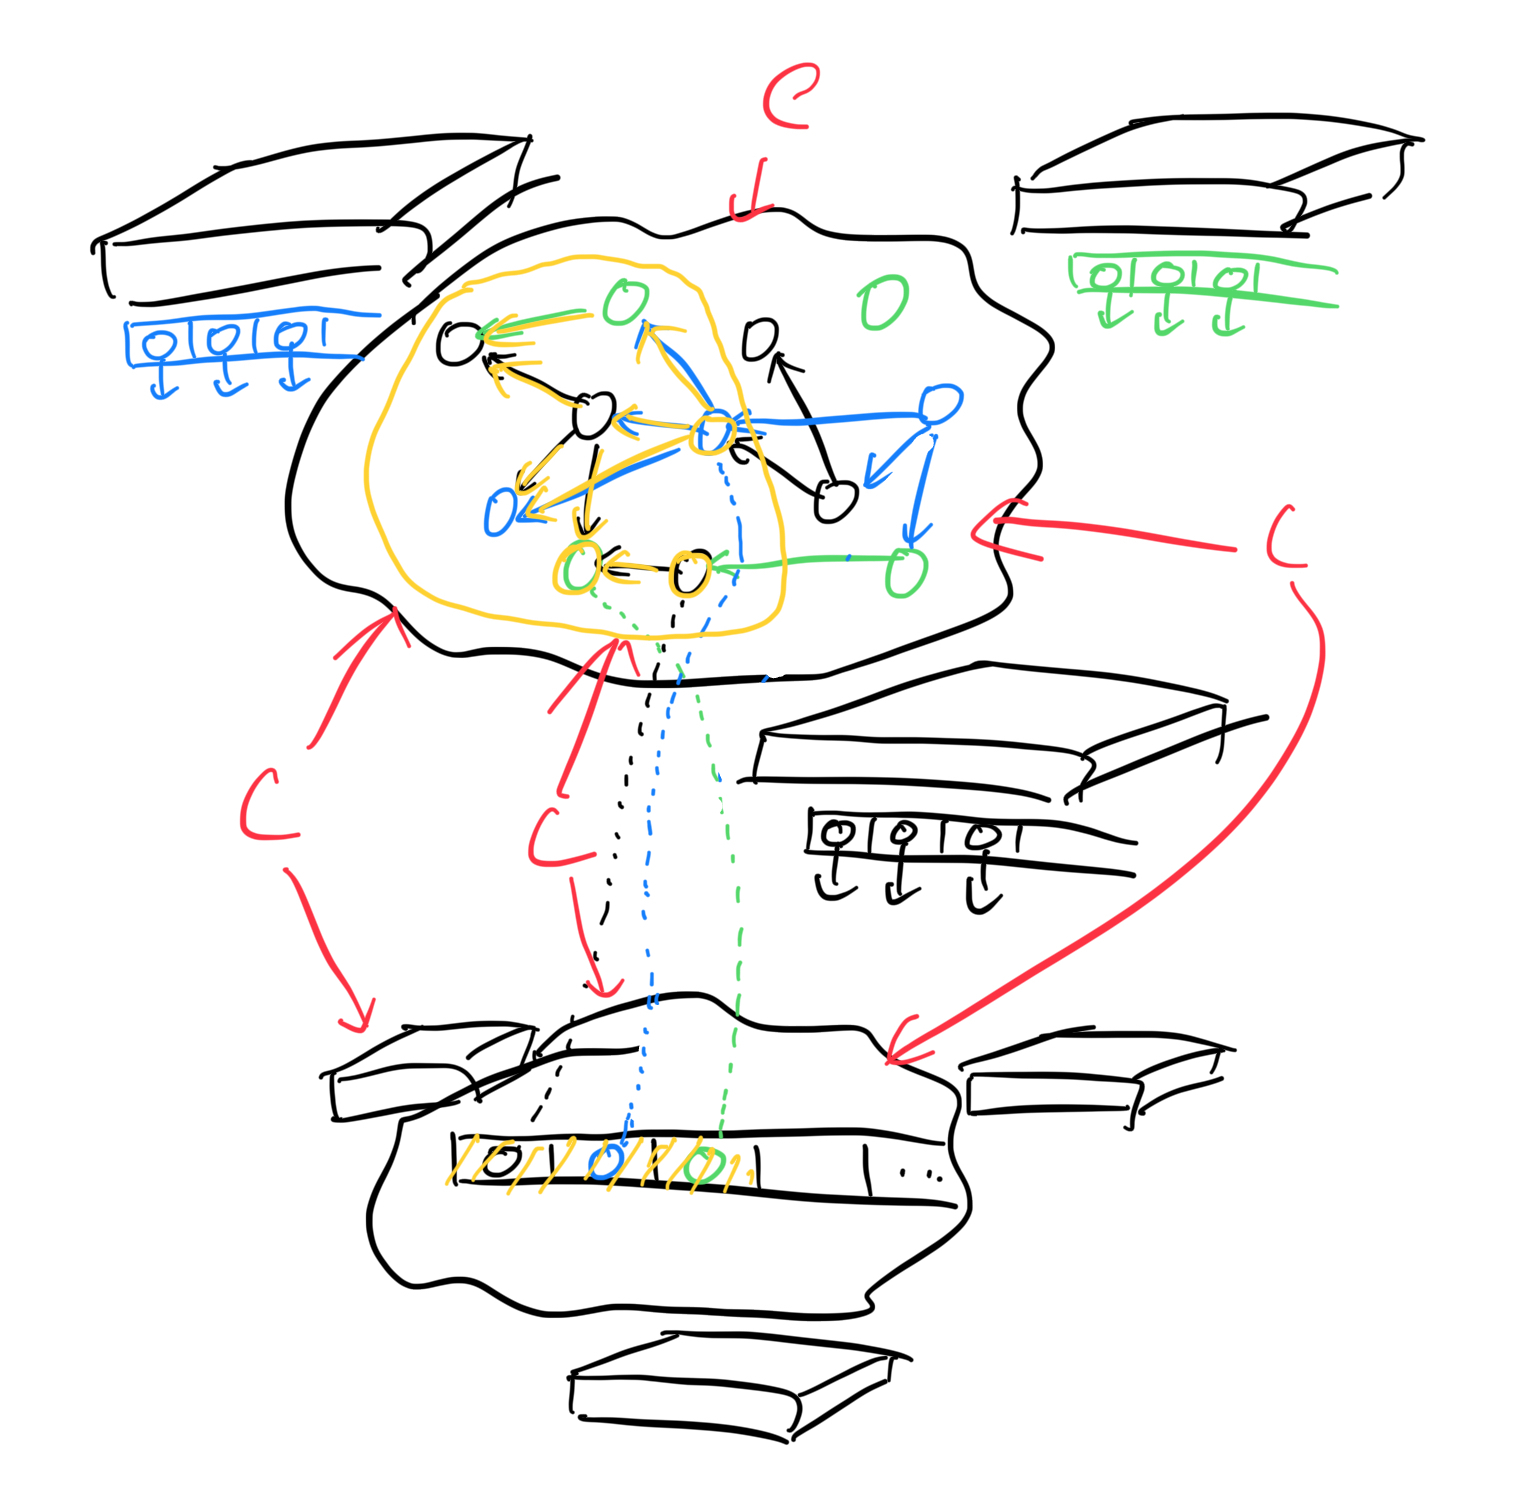
\includegraphics[width=300pt]{graphs/IMG_0057}
    \caption{The finalized reasoning is marked in yellow.}
    \Description{}
\end{figure}

Notice some intents are reordered when submitting to consensus.
This is unavoidable as the submissions are distributed.
However, it does not affect the outcome, which is what makes \sys substantially different from a rollup.
\sgd{Necessary to discuss rollup more formly?}
As we stated earlier, the consensus is retired from an ordering mechanism, but purely for finality.
The ordering without shared state is completely \emph{offloaded} into \sys.